%! TeX root = ../../main-en.tex
% 译自: backmatter/zh/appendix_b.tex @ 9048155:backmatter/zh/appendix_b.tex
\chapter{Programmers' \texorpdfstring{``Holy Wars''}{“Holy Wars”}}
\label{app:holy-wars}

Programmers are, on the whole, reasonable people. But bring up where the curly brace should go, how many spaces to indent, or which editor to use, and even the most reasonable of them go red in the face. Some of these arguments have been running for decades without a winner. Programmers, laughing at themselves, call them \emph{holy wars}.\lazynote{Holy war}{Programmer slang for an argument that has no right answer but can go on for decades.}

This appendix tells the story of a few of the most famous holy wars. Let us agree on one thing up front: most of them have no right or wrong side. The louder the shouting, the more likely it is that both sides have a point.

\section{It All Started with an Egg}

The phrase ``holy war'' caught on in computing thanks to a paper published on 1~April 1980: Danny Cohen's \emph{On Holy Wars and a Plea for Peace}. Its first sentence reads: ``This is an attempt to stop a war.''

The ``war'' Cohen had in mind is byte order, which we met in Section~\ref{sec:mem-street}: when a number takes up several bytes, do you store (or send) its low byte first, or its high byte? In the early days of networking, people argued about this endlessly. Cohen borrowed two words from \emph{Gulliver's Travels}. There, Lilliput and its neighbour fight a long and bloody war over which end of a boiled egg should be cracked first, the small end or the big end; the two parties are called the Little-Endians and the Big-Endians (Figure~\ref{fig:eggs}). Ever since, ``little-endian'' and ``big-endian'' have been computer terms.

\begin{figure}[htbp]
  \centering
  \begin{tikzpicture}[line width=0.8pt]
    \foreach \x/\s/\who/\say in {0/1/Little-Endians/{Small end first!}, 6.0/-1/Big-Endians/{Big end first!}} {
      \begin{scope}[shift={(\x,0)}]
        % a Lilliputian
        \draw (0,1.6) circle (0.22);
        \draw (0,1.38) -- (0,0.6);
        \draw (0,0.6) -- (-0.2,0) (0,0.6) -- (0.2,0);
        \draw (0,1.2) -- (\s*0.55,1.35);
        \draw (0,1.2) -- (-\s*0.35,0.9);
        % the egg
        \filldraw[fill=yellow!15] (\s*0.9,1.4) ellipse (0.32 and 0.22);
        \fill[orange!70] (\s*1.2,1.4) circle (0.05);   % the end to crack first
        \node[font=\small] at (0,-0.35) {\who};
        \node[draw, rounded corners, fill=white, font=\small] at (\s*0.4,2.45) {\say};
      \end{scope}
    }
    \node[font=\Large\bfseries, text=lazyred] at (3.0,1.2) {VS};
    \draw[gray, line width=1pt] (-1.2,0) -- (7.2,0);
  \end{tikzpicture}
  \caption{The egg war in \emph{Gulliver's Travels}, which gave the byte-order war its name}
  \label{fig:eggs}
\end{figure}

Today, x86 and RISC-V are both little-endian, while data sent over a network is big-endian by convention (which is why big-endian is also called ``network byte order''). Nobody won this war; everyone just learned to live together. When you need to, you convert, and that is that.

\section{Where Does the Brace Go?}

C uses curly braces \texttt{\{\}} to group code into a block, but it says nothing about where the opening brace should go. And so several ``schools'' were born:

\begin{minted}[linenos=false]{c}
/* K&R style: opening brace at the end of the line */
if (x > 0) {
    y = 1;
}

/* Allman style: opening brace on a line of its own */
if (x > 0)
{
    y = 1;
}

/* GNU style: braces indented 2, the code inside another 2 */
if (x > 0)
  {
    y = 1;
  }
\end{minted}

\begin{itemize}
  \item \textbf{K\&R style} comes from \emph{The C Programming Language}, the book by Kernighan and Ritchie, the fathers of C. It is the style used in this book.
  \item \textbf{Allman style} is named after Eric Allman, the author of many BSD programs (sendmail, the mail server, for one). Its advantage is that the opening and closing braces line up vertically, so you can see at a glance which two belong together.
  \item \textbf{GNU style} is what the GNU project's coding standards prescribe. Most people do a double take the first time they see it.
\end{itemize}

The Linux kernel is firmly on the K\&R side, and it does not hide it. Its coding style says: for most statements, put the opening brace at the end of the line; functions are the only exception, where the opening brace goes at the beginning of the next line. ``Heretic people all over the world have claimed that this inconsistency is \ldots{} well \ldots{} inconsistent, but all right-thinking people know that (a) K\&R are \emph{right} and (b) K\&R are right.''\lazynote{Why functions are different}{The kernel's own reason: you can't nest functions in C, so functions are special anyway. Another common explanation: early C wrote the parameter types between the closing parenthesis and the opening brace.} As for GNU style, the document opens with this: ``First off, I'd suggest printing out a copy of the GNU coding standards, and NOT read it. Burn them, it's a great symbolic gesture.''

\begin{figure}[htbp]
  \centering
  \begin{tikzpicture}[line width=0.8pt]
    \foreach \x/\s/\brace/\say in {0/1/{if (x) \{}/{End of the line!}, 5.6/-1/{\{}/{Next line!}} {
      \begin{scope}[shift={(\x,0)}]
        \draw (0,1.6) circle (0.22);
        \draw (0,1.38) -- (0,0.6);
        \draw (0,0.6) -- (-0.2,0) (0,0.6) -- (0.2,0);
        \draw (0,1.2) -- (\s*0.5,1.5);
        \draw (0,1.2) -- (-\s*0.3,0.85);
        \node[font=\ttfamily\bfseries\huge, text=lazyred] at (\s*0.95,1.75) {\{};
        \node[draw, rounded corners, fill=white, font=\small] at (\s*0.2,2.6) {\say};
      \end{scope}
    }
    \node[font=\small, gray, align=center] at (2.8,0.6) {Round 1\,000\,000};
    \draw[gray, line width=1pt] (-1.0,0) -- (6.6,0);
  \end{tikzpicture}
  \caption{The brace war}
  \label{fig:braces}
\end{figure}

\section{Naming Things}

There is an old saying in computing, usually credited to Phil Karlton: ``There are only two hard things in Computer Science: cache invalidation and naming things.'' Naming functions and variables is a holy war of its own.

\subsection{The Microsoft Way}

The Windows driver in Chapter~\ref{chap:c-structure} is full of names like \texttt{ZwCreateFile}, \texttt{ExAllocatePool2} and \texttt{IO\_STATUS\_BLOCK}. In the Windows kernel, every word in a function name starts with a capital letter (this is called PascalCase), and in front goes a prefix of two or three letters saying which part of the kernel the function belongs to: \texttt{Io} is the I/O manager, \texttt{Ke} the kernel core, \texttt{Mm} the memory manager, \texttt{Ex} the executive, \texttt{Ob} the object manager, and so on.

So what does \texttt{Zw} stand for? The answer is a surprise: \textbf{nothing at all}.\lazyhint{You will find claims online that Zw means ``Zero Wait'' and the like. They are all guesses; Microsoft has never confirmed any of them.} Microsoft's documentation says so plainly: ``The Nt prefix is an abbreviation of Windows NT, but the Zw prefix has no meaning.'' The letters were chosen partly to avoid clashing with other APIs, and partly to avoid using up a two-letter prefix that might be useful one day. When Raymond Chen, a long-time Microsoft engineer, answered the question on his blog, \emph{The Old New Thing}, a single word was enough: ``Nothing.''

Microsoft has an even more famous naming habit: \emph{Hungarian notation}. You put a short lowercase prefix in front of a variable name to say what type it is: \texttt{dwFlags} is a DWORD, \texttt{lpszName} is a ``long pointer to a zero-terminated string'', and \texttt{hWnd} is a handle to a window. It was invented by Charles Simonyi at Microsoft, who is Hungarian---hence the name.\lazynote{Hungarian notation}{Putting a prefix that describes the variable in front of its name. Named after its inventor, Charles Simonyi, who is Hungarian.} What Simonyi originally meant was for the prefix to show what a variable is \emph{for} (a row number or a column number, say). Many people later used it to show the variable's \emph{type} instead, and that turned it into dead weight.

\subsection{The Linux Way}

In the Linux and Unix world, names are all lowercase, with underscores between the words (this is called snake\_case): \texttt{copy\_from\_user}, \texttt{count\_active\_users}. The Linux kernel coding style says: ``C programmers do not use cute names like \texttt{This\-Variable\-Is\-A\-Temporary\-Counter}. A C programmer would call that variable \texttt{tmp}, which is much easier to write, and not the least more difficult to understand.'' And on Hungarian notation it does not mince words: ``Encoding the type of a function into the name (so-called Hungarian notation) is asinine---the compiler knows the types anyway and can check those, and it only confuses the programmer.''

Still, Unix has no function called \texttt{create\_file}. To open or create a file you use \texttt{open}, and there is also a system call just for creating files, called \texttt{creat}---one \texttt{e} short. Kernighan and Pike tell the story in \emph{The UNIX Programming Environment} (1984): Ken Thompson, one of the inventors of Unix, was once asked what he would do differently if he were redesigning the system. His reply: ``I'd spell creat with an e.'' Decades later, Thompson helped design the Go language, and in Go's standard library the name is finally spelled \texttt{O\_CREATE}.

\section{How Wide an Indent?}

Every community has its own rule for indent width (Table~\ref{tab:indent}).

\begin{table}[htbp]
  \begin{lazywide}
  \caption{Indent widths around the world}
  \label{tab:indent}
  \begin{tabular}{cL{4.2cm}L{6.4cm}}
    \toprule
    Width & Who uses it & Notes \\
    \midrule
    8 & The Linux kernel & Indents with tabs; a tab is 8 columns wide \\
    4 & Python (PEP 8), the C code in this book & Python marks blocks by indentation, so a wrong indent means a wrong program \\
    2 & GNU C code, Google's C++ style guide, Ruby, Lisp & Deeply nested code does not get pushed off the right edge so easily \\
    3 & Verilog (when edited in Emacs) & Emacs's verilog-mode sets \texttt{verilog-indent-level} to 3 by default \\
    \bottomrule
  \end{tabular}
  \end{lazywide}
\end{table}

Verilog's 3-space indent is an interesting case. The Verilog language itself says nothing about indentation. But many chip designers write their Verilog in Emacs, and Emacs's verilog-mode indents by 3 by default. Enough people used it that 3 spaces became the look of the code at quite a few chip companies. One editor's default setting quietly decided the habit of a whole industry.

The Linux kernel, as usual, leaves no room for doubt: ``Tabs are 8 characters, and thus indentations are also 8 characters. There are heretic movements that try to make indentations 4 (or even 2!) characters deep, and that is akin to trying to define the value of PI to be 3.'' With 8-column indents, three or four levels of nesting push the code over to the right. The style guide says that is exactly the point: ``if you need more than 3 levels of indentation, you're screwed anyway, and should fix your program.'' It is the same idea as in Chapter~\ref{chap:c-structure}: let the success path run straight down the page instead of nesting deeper and deeper.

\section{\texorpdfstring{\NoCaseChange{Tabs}}{Tabs} or Spaces?}

Should you indent with tabs or with spaces? This may be the oldest and fiercest holy war of them all.

\begin{minted}[linenos=false]{text}
Indented with a tab (one character, 0x09, drawn here as ------->):
if (x > 0) {
------->y = 1;
}

Indented with 4 spaces (four characters, 0x20, drawn here as .):
if (x > 0) {
....y = 1;
}
\end{minted}

\textbf{Team Tab} says: one level of indent is one tab, which is clear and meaningful. Everyone can set the tab width they like in their own editor and read the code the way they find comfortable. And the files are smaller, too.

\textbf{Team Space} says: but that is exactly the problem. Because everyone's tabs are a different width, code that lines up perfectly in your editor is a crooked mess in mine. With spaces, it looks the same everywhere.

Worst of all is mixing the two. Python uses indentation to mark blocks, so mixing tabs and spaces can change what a program means. Python~3 simply refuses: if tabs and spaces are mixed inconsistently, you get an error (\texttt{TabError}).

\paragraph{Makefiles: tabs and nothing else.}
\lazyhint{All because one programmer did not want to upset a dozen friends, programmers everywhere have had to remember for decades: Makefiles need tabs.}In every Makefile in this book, each command line \emph{must} start with a tab. Use spaces and \texttt{make} will give you an error. Why such an awkward rule? Stuart Feldman, the author of make, explained it later (as quoted in Eric Raymond's \emph{The Art of Unix Programming}): ``Why the tab in column 1? Yacc was new, Lex was brand new. I hadn't tried either, so I figured this would be a good excuse to learn. After getting myself snarled up with my first stab at Lex, I just did something simple with the pattern newline-tab. It worked, it stayed. And then a few weeks later I had a user population of about a dozen, most of them friends, and I didn't want to screw up my embedded base. The rest, sadly, is history.''

\paragraph{Do people who use spaces earn more?}
In 2017, David Robinson, a data scientist at Stack Overflow, analysed that year's developer survey and published an article that caused quite a stir: \emph{Developers Who Use Spaces Make More Money Than Those Who Use Tabs}. Among more than 12\,000 professional developers who reported their salary, the median salary of those who used spaces was \$59\,140, against \$43\,750 for those who used tabs. Even after taking country, years of experience, programming language and so on into account, using spaces was still associated with an 8.6\% higher salary. Robinson himself pointed out, of course, that this is correlation, not causation. Swapping your tabs for spaces will not get you a pay rise.

Even television has made fun of this war. In the TV series \emph{Silicon Valley}, the main character, Richard, breaks up with his girlfriend because she indents with spaces.

\begin{figure}[htbp]
  \centering
  \begin{tikzpicture}[line width=0.7pt]
    % one line of code, cell by cell
    \foreach \i in {0,...,11} \draw[gray!50] (\i*0.55,0) rectangle +(0.55,0.55);
    \foreach \i/\c in {8/y, 9/=, 10/1, 11/;} \node[font=\ttfamily] at (\i*0.55+0.275,0.275) {\c};
    \fill[lazyred!20] (0,0.62) rectangle (4.4,1.0);
    \node[font=\footnotesize] at (2.2,0.81) {Tab: 1 character, 8 columns};
    \begin{scope}[shift={(0,-1.1)}]
      \foreach \i in {0,...,11} \draw[gray!50] (\i*0.55,0) rectangle +(0.55,0.55);
      \foreach \i in {0,...,3} \node at (\i*0.55+0.275,0.275) {.};
      \foreach \i/\c in {4/y, 5/=, 6/1, 7/;} \node[font=\ttfamily] at (\i*0.55+0.275,0.275) {\c};
      \node[font=\small, anchor=west, align=left] at (6.8,0.275) {4 spaces:\\4 characters, 4 columns};
    \end{scope}
    \node[draw, rounded corners, fill=white, font=\small] at (8.2,1.2) {Worth a break-up?};
  \end{tikzpicture}
  \caption{Tabs and spaces}
  \label{fig:tabs}
\end{figure}

\section{\texorpdfstring{\NoCaseChange{Vim}}{Vim} versus \texorpdfstring{\NoCaseChange{Emacs}}{Emacs}}

If there is one holy war that makes every programmer pick a side, it is the \emph{editor war}: vi or Emacs?

Both editors were born in 1976. vi was written by Bill Joy at Berkeley (yes, the BSD people again). Later came the more powerful Vim (Vi IMproved), released in 1991 by the Dutch programmer Bram Moolenaar, who maintained it until his death in 2023. Emacs started life as a set of editing macros written by Richard Stallman and Guy Steele; later Stallman wrote GNU Emacs, one of the very first pieces of the GNU project.

The two editors think in completely different ways. vi has \emph{modes}: in normal mode every key is a command, and to type text you first press \texttt{i} to enter insert mode. Emacs has no modes; its commands are key combinations with Ctrl, Alt and friends. It also has a whole Lisp language built in, so you can add anything to it: read your mail, play games, browse the web\ldots{}

That gave each side plenty to make fun of:
\begin{itemize}
  \item The vi camp says: Emacs is a great operating system, lacking only a decent editor.
  \item ``Emacs'' stands for Escape-Meta-Alt-Control-Shift---far too many keys to press. (The vi camp made that one up.)
  \item Stallman gave himself a holy title: St.~IGNUcius of the Church of Emacs. He says that ``vi vi vi'' is the editor of the beast---in Roman numerals, vi is 6, so vi vi vi is 666. He adds, though, that using a free version of vi is not a sin; it is a penance.
\end{itemize}

vi's most famous ``feature'' is that beginners who get in cannot get out. In 2012, someone asked on Stack Overflow: ``How do I exit the Vim editor?'' By 2017 the question had helped more than a million people; by 2019 it had been viewed over two million times. The answer is simple, really: press \texttt{Esc}, type \texttt{:q!}, and press Enter.

\begin{figure}[htbp]
  \centering
  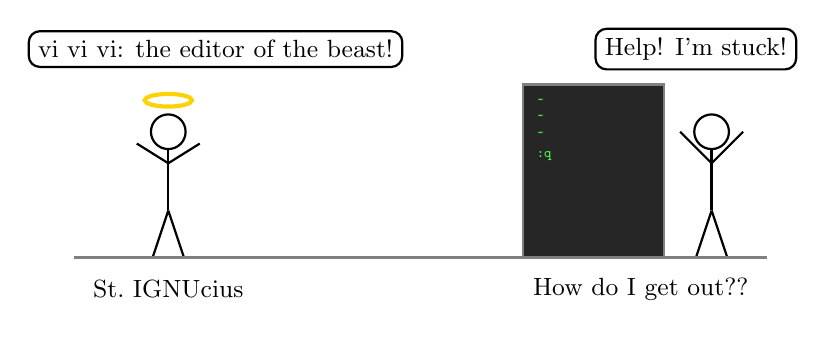
\begin{tikzpicture}[line width=0.8pt]
    % St. IGNUcius
    \draw (0,1.6) circle (0.22);
    \draw[yellow!70!orange, line width=1.5pt] (0,2.0) ellipse (0.3 and 0.08);
    \draw (0,1.38) -- (0,0.6);
    \draw (0,0.6) -- (-0.2,0) (0,0.6) -- (0.2,0);
    \draw (0,1.2) -- (0.4,1.45) (0,1.2) -- (-0.4,1.45);
    \node[font=\small, align=center] at (0,-0.4) {St.~IGNUcius};
    \node[draw, rounded corners, fill=white, font=\small] at (0.6,2.65) {vi vi vi: the editor of the beast!};
    % someone trapped in Vim
    \begin{scope}[shift={(5.4,0)}]
      \filldraw[fill=black!85, draw=gray] (-0.9,0) rectangle (0.9,2.2);
      \node[font=\ttfamily\tiny, text=green!70, anchor=north west, align=left] at (-0.85,2.15)
        {\textasciitilde\\\textasciitilde\\\textasciitilde\\:q};
      \draw (1.5,1.6) circle (0.22);
      \draw (1.5,1.38) -- (1.5,0.6);
      \draw (1.5,0.6) -- (1.3,0) (1.5,0.6) -- (1.7,0);
      \draw (1.5,1.2) -- (1.1,1.6) (1.5,1.2) -- (1.9,1.6);
      \node[font=\small, align=center] at (0.6,-0.4) {How do I get out??};
      \node[draw, rounded corners, fill=white, font=\small] at (1.3,2.65) {Help! I'm stuck!};
    \end{scope}
    \draw[gray, line width=1pt] (-1.2,0) -- (7.6,0);
  \end{tikzpicture}
  \caption{The editor war}
  \label{fig:editors}
\end{figure}

By the way, this book was written in Vim. Whether the author has ever secretly used Emacs, we will not say.

\section{And There Are More}

There are many more holy wars than these. Here are a few other famous ones:

\begin{itemize}
  \item \textbf{Is \texttt{goto} harmful?} Dijkstra's 1968 letter \emph{Go To Statement Considered Harmful} kept people arguing for decades. As we saw in Chapter~\ref{chap:c-structure}, a \texttt{goto} that only jumps to the end of a function actually makes code clearer.
  \item \textbf{Do indexes start at 0 or 1?} Array indexes in C start at 0; in Fortran, Lua and MATLAB they start at 1. In 1982, Dijkstra wrote a short note just about this: \emph{Why numbering should start at zero}.
  \item \textbf{\texttt{int *p} or \texttt{int* p}?} The first says ``\texttt{*p} is an \texttt{int}''; the second says ``the type of \texttt{p} is \texttt{int*}''. But in \texttt{int* p, q;} only \texttt{p} is a pointer---\texttt{q} is a plain \texttt{int}. That is the \texttt{int *p} camp's favourite example.
  \item \textbf{Yoda conditions.} To guard against writing \texttt{=} when you meant \texttt{==} (Section~\ref{sec:logic}), some people put the constant on the left: \texttt{if (5 == n)}. Mistype it as \texttt{5 = n}, and the compiler stops you with an error. Critics say this reads like Yoda from \emph{Star Wars} talking (``if five equals n\ldots''), and that with compiler warnings there is no need for the contortion.
  \item \textbf{Line endings: CRLF or LF?} An old teletype needed two actions to start a new line: a carriage return (CR, move the print head back to the start of the line) and a line feed (LF, roll the paper up one line). Windows kept both characters, \texttt{\textbackslash r\textbackslash n}; Unix uses just \texttt{\textbackslash n}. This one bit us while writing this book: a few files got saved with CRLF, and the scripts failed when we ran them in WSL.
  \item \textbf{Microkernel or monolithic kernel?} In 1992, Andrew Tanenbaum, an operating systems professor and the author of Minix, posted to a newsgroup under the title \emph{LINUX is obsolete}. He criticised Linux for putting everything into one big kernel, an outdated design in his view. Linus Torvalds, the student who had just written Linux, fired straight back. The debate went down in operating systems history---and Linux went on to become the most widely used kernel in the world.
  \item \textbf{How do you say GIF?} Steve Wilhite, the inventor of the image format, accepted an award in 2013 with a single line on the screen: it's pronounced ``jif'' (like the peanut butter brand Jif). Most people still say ``gif'' (as in ``gift''). Not even the inventor could end this war.
\end{itemize}

\section{How to End a Holy War}

Most of these arguments have no right or wrong answer---only habits and trade-offs. What really matters is the rule from Chapter~\ref{chap:c-structure}: \textbf{be consistent with the code around you}. Everyone in a project using the same style matters far more than which style it is.

Today, many projects simply hand the decision to a tool. Go comes with \texttt{gofmt}, and all Go code is laid out its way, so there is nothing to argue about. C and C++ have \texttt{clang-format}, Python has \texttt{black}: put a config file in the project, and the code is formatted automatically when you save. Let the machine decide where the braces go, and people are free to argue about something else.

Such as: Vim or Emacs---which one is better?
